\chapter{Implementacija i korisničko sučelje}


\section{Korištene tehnologije i alati}

Za komunikaciju u timu korištene su aplikacije \underline{WhatsApp}\footnote{\url{https://www.whatsapp.com/}} i \underline{Discord}\footnote{\url{https://discord.com/}}. Na web platformi \underline{GitLab}\footnote{\url{https://gitlab.com}} nalazi se udaljeni repozitorij projekta, a kao sustav za upravljanje izvornim kodom korišten je \underline{Git}\footnote{\url{https://git-scm.com/}}. Za razvoj su korištena dva razvojna okruženja, \underline{Microsoft Visual Studio Code}\footnote{\url{https://visualstudio.microsoft.com/}} i \underline{Intellij IDEA}\footnote{\url{https://www.jetbrains.com/idea/}}. Microsoft Visual Studio Code je integrirano razvojno okruženje tvrtke Microsoft, a koristi se za razvoj računalnih programa, web stranica, web aplikacija, web usluga i mobilnih aplikacija. IntelliJ IDEA integrirano je razvojno okruženje napisano u Javi za razvoj računalnog softvera, razvio ga je JetBrains, a dostupan je kao izdanje licenci za zajednicu Apache 2 i u vlastitom komercijalnom izdanju. \par		
Aplikacija je napisana koristeći aplikacijski okvir \underline{Spring Framework}\footnote{\url{https://spring.io/}} i jezik \underline{Java}\footnote{\url{https://www.java.com/en/}} za izradu backenda. Spring je skup biblioteka i alata koji olakšava razvoj aplikacija te čini programiranje u Javi bržim, lakšim i sigurnijim. Usredotočenost Springa na brzinu, jednostavnost i produktivnost učinila ga je najpopularnijim okvirom za Javu. Za lakše uključivanje i integriranje modula, postavljanje securityja i mapiranje objektnog modela na relacijsku bazu podataka korišten je Spring Boot. \underline{Spring Boot  }\footnote{\url{https://spring.io/projects/spring-boot/}} radi automatsko podešavanja i povezivanje različitih modula tako da analizira što smo uključili u classpath te sam zaključuje kako te module povezati u smislenu cjelinu. Za razvoj Web servisa korišten je \underline{REST}. REST, ili REpresentational State Transfer, arhitekturalni je stil za razvoj Web servisa koji pruža standard između računalnih sustava na webu, olakšavajući njihovu međusobnu komunikaciju. \par
Za praćenje promjena u bazi podataka korišten je \underline{Liquibase}\footnote{\url{https://www.liquibase.org/}}. Liquibase je knjižnica sa neovisnom bazom podataka otvorenog koda za praćenje, upravljanje i primjenu promjena sheme baze podataka. Pokrenut je 2006. godine kako bi omogućio lakše praćenje promjena u bazama podataka. Sve promjene u bazi podataka pohranjuju se u tekstualne datoteke (XML, JSON) i identificiraju se kombinacijom oznake "id" i "author", kao i imenom same datoteke. Za upravljanje bazom podataka korišten je besplatan sustav \underline{PostgreSQL}\footnote{\url{https://www.postgresql.org/}} koji poštuje ACID principe pri izvođenju transakcija. Za testiranje backenda korišten je jednostavan okvir za pisanje ponovljivih testova \underline{JUnit}\footnote{\url{https://junit.org/}}. JUnit je instanca xUnit arhitekture za okvire za jedinstveno testiranje. \par
Za izradu frontenda korišten je JavaScript library \underline{React}\footnote{\url{https://reactjs.org/}} i jezik \underline{TypeScript}\footnote{\url{https://www.typescriptlang.org/}}. React se koristi za izgradnju korisničkog sučelja ili UI komponenti. Održava ga Facebook. React se može koristit kao osnova u razvoju aplikacija. Za realizaciju pojedinih prikaza kao što su okviri za prijavu i registraciju, tablice za statistiku, gumbi i slično, korišten je \underline{Material-UI}\footnote{\url{https://material-ui.com/}}. To je open-source projekt koji sadrži React komponente koje implementiraju Googleov Material Design. Za preuzimanje rasporeda šetnji korišten je React-pdf koji služi za jednostavno generiranje PDF datoteka. HTTP zahtjevi i odgovori ostvareni su korištenjem \underline{Axios-a}\footnote{\url{https://www.npmjs.com/package/axios}}. Axios je vrlo popularan JavaScript library za izvršavanje HTTP zahtjeva. Podržava starije i sve moderne preglednike, radi u Node.js-u te provodi automatsku transformaciju JSON podataka. Temelji se na obećanjima, što omogućuje pisanje async/await koda za vrlo lako izvršavanje XHR zahtjeva. Dizajn web aplikacije napravljen je pomoću stilskog jezika \underline{CSS}\footnote{\url{https://www.w3.org/Style/CSS/Overview.en.html}}. Testiranje frontenda ostvareno je koristeći radni okvir \underline{Selenium}\footnote{\url{https://www.selenium.dev/}}. \par
Dokumentacija je napisana u jeziku \underline{LaTex}\footnote{\url{https://www.latex-project.org/}} u integriranom okruženju za pisanje \underline{TeXStudio}\footnote{\url{https://www.texstudio.org/}}. Za izradu UML dijagrama korišten je alat \underline{Astah UML}\footnote{\url{https://astah.net/downloads/}}. ER dijagram baze podataka izrađen je u besplatnom online softveru \underline{draw.io}\footnote{\url{https://app.diagrams.net/}}, koji se između ostalog koristi i za izradu dijagrama toka i procesa, organizacijskih dijagrama, UML, ER i mrežnih dijagrama.



\eject 

\section{Ispitivanje programskog rješenja}

	\subsection{Ispitivanje komponenti}

	
	\noindent Za testiranje smo odabrali WalkController i AssociationController koji implementiraju glavne funkcionalnosti sustava. Testirali smo controllere kako bi provjerili rad sustava u cjelini. Prije testova postavljeni su testni podaci. Na slici je prikazano postavljanje Spring Boot Security podataka.

	\begin{figure}[H]
		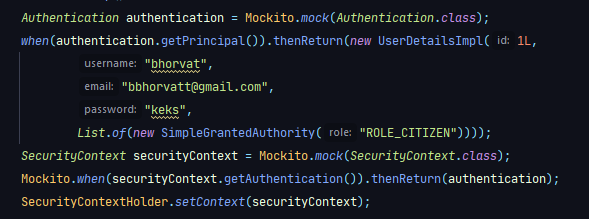
\includegraphics[width=\linewidth]{slike/Testovi-1.png}
		\centering
		\caption{Postavljanje sigurnosti}
		\label{fig:testovi1}
	\end{figure}

	\noindent Zbog testiranja prijave šetnje u prošlom vremenu, postavili smo fiksni datum kako je prikazano na slici dolje. Zbog vremenskih zona zahtjevi koji se šalju su u vremenskoj zoni GMT+0, a u sustavu se pohranjuju u vremenskoj zoni GMT+1.

	\begin{figure}[H]
		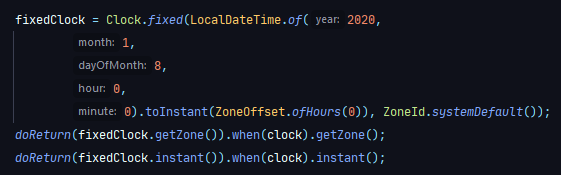
\includegraphics[width=\linewidth]{slike/Testovi-2.png}
		\centering
		\caption{Postavljanje fiksnog vremena}
		\label{fig:testovi2}
	\end{figure}

	\eject

	\noindent Zbog testiranja prijave šetnje kad je pas već zauzet, potrebna su nam dva građana.

	\begin{figure}[H]
		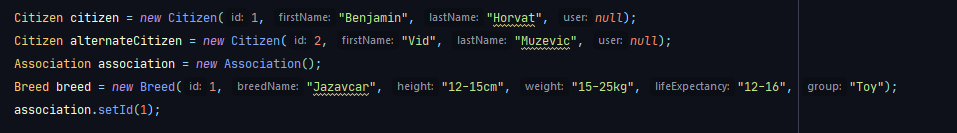
\includegraphics[width=\linewidth]{slike/Testovi-3.png}
		\centering
		\caption{Postavljanje 2 građana, 1 udruge i 1 pasmine}
		\label{fig:testovi3}
	\end{figure}

	\noindent Postavili smo testne podatke za dva psa koji su predodređeni za pojedinačnu šetnju i dva psa koji su predodređeni za grupnu šetnju. Zatim su postavljeni podaci za pet šetnji sa prije definiranim životinjama.

	\begin{figure}[H]
		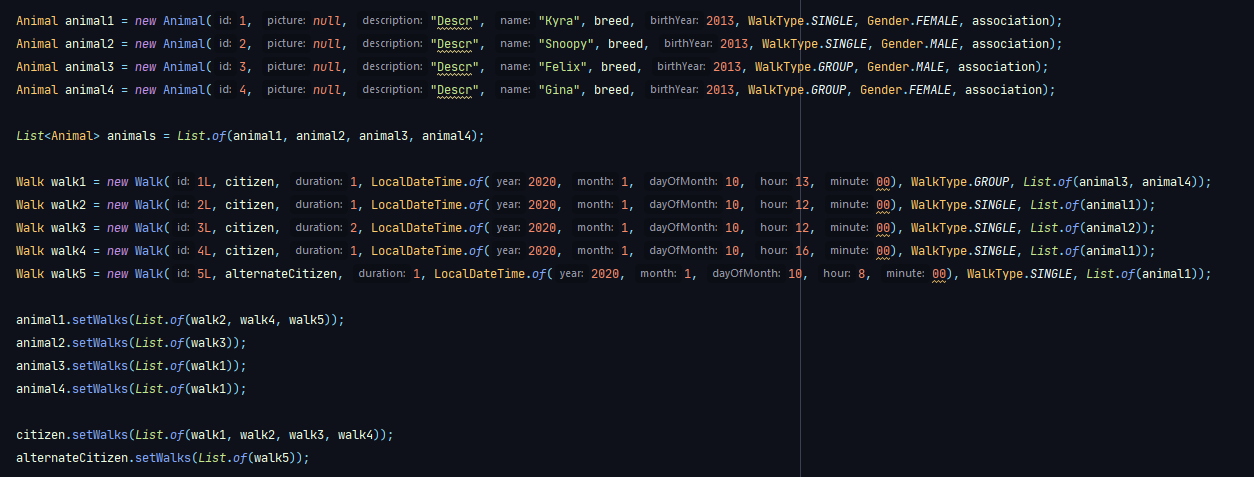
\includegraphics[width=\linewidth]{slike/Testovi-4.png}
		\centering
		\caption{Postavljanje životinja i šetnji}
		\label{fig:testovi4}
	\end{figure}
	
	\eject

	\noindent Postavljanje ponašanja dvojnika za navedene pozive metoda AnimalRepositoryja.

	\begin{figure}[H]
		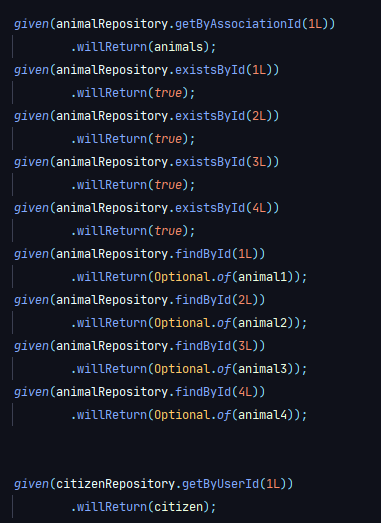
\includegraphics[width=\linewidth]{slike/Testovi-5.png}
		\centering
		\caption{Postavljanje dvojnika}
		\label{fig:testovi5}
	\end{figure}

	\noindent Na API poziv "/api/walk" šaljemo ispravne podatke šetnje. Očekivani rezultat je statusni kod 200.

	\begin{figure}[H]
		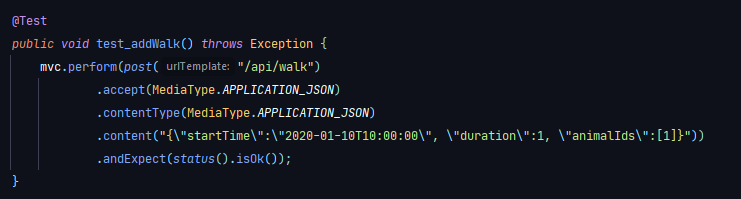
\includegraphics[width=\linewidth]{slike/Testovi-6.png}
		\centering
		\caption{Testiranje ispravne šetnje}
		\label{fig:testovi6}
	\end{figure}

	\noindent Na API poziv "/api/walk" šaljemo početak šetnje koji je prošao. Očekivani rezultat je statusni kod 400.

	\begin{figure}[H]
		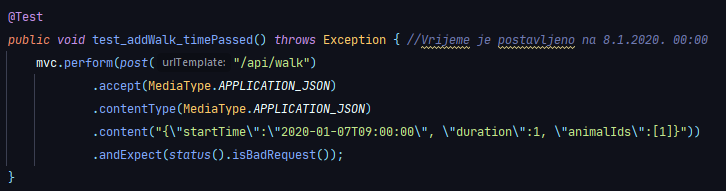
\includegraphics[width=\linewidth]{slike/Testovi-7.png}
		\centering
		\caption{Testiranje šetnje u prošlom vremenu}
		\label{fig:testovi7}
	\end{figure}
	
	\noindent Na API poziv "/api/walk" šaljemo podatke o šetnji u terminu u kojem je građanin već zauzet. Očekivani rezultat je statusni kod 400.

	\begin{figure}[H]
		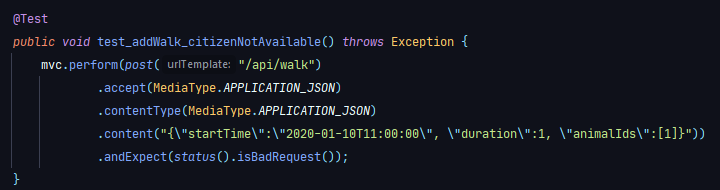
\includegraphics[width=\linewidth]{slike/Testovi-8.png}
		\centering
		\caption{Testiranje šetnje za koju građanin nije dostupan}
		\label{fig:testovi8}
	\end{figure}

	\noindent Na API poziv "/api/walk" šaljemo podatke o šetnji bez navedene životinje. Očekivani rezultat je statusni kod 400.

	\begin{figure}[H]
		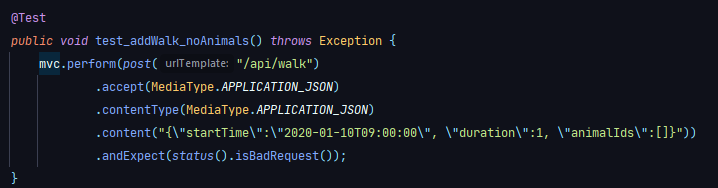
\includegraphics[width=\linewidth]{slike/Testovi-9.png}
		\centering
		\caption{Testiranje šetnje bez odabrane životinje}
		\label{fig:testovi9}
	\end{figure}

	\noindent Na API poziv "/api/walk" šaljemo podatke o šetnji u terminu u kojem je životinja već zauzeta. Očekivani rezultat je statusni kod 400.
	
	\begin{figure}[H]
		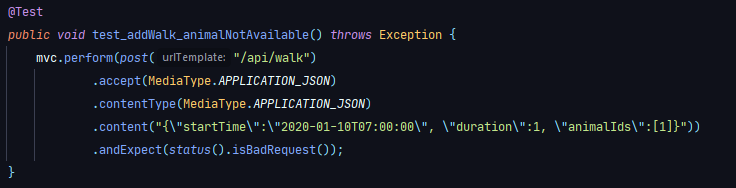
\includegraphics[width=\linewidth]{slike/Testovi-10.png}
		\centering
		\caption{Testiranje šetnje za koju životinja nije dostupna}
		\label{fig:testovi10}
	\end{figure}

	\eject

	\noindent Na API poziv "/api/walk/animals" šaljemo podatke o željenom početku šetnje, trajanju i odabranu udrugu. Cilj nam je provjeriti dostupnost životinje u navedenom terminu. Očekivani rezultat je statusni kod 200.

	\begin{figure}[H]
		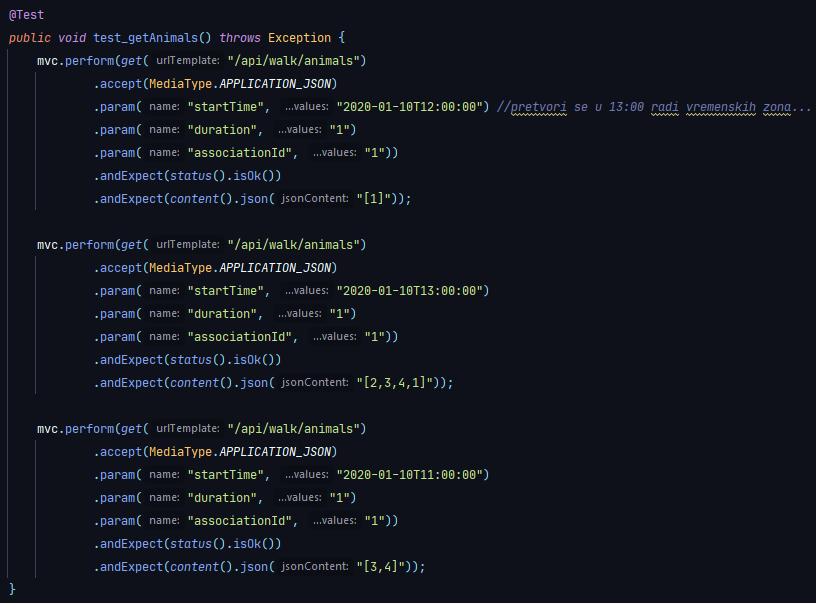
\includegraphics[width=\linewidth]{slike/Testovi-11.png}
		\centering
		\caption{Testiranje dostupnosti životinja}
		\label{fig:testovi11}
	\end{figure}

	\eject

	\noindent Slijede rezultati navedenih testova.

	\begin{figure}[H]
		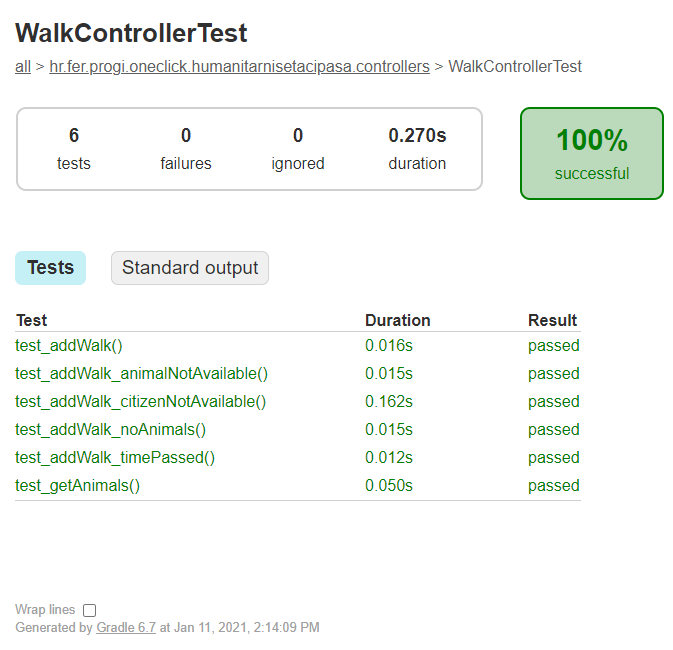
\includegraphics[width=\linewidth]{slike/Testovi-16.png}
		\centering
		\caption{Rezultati testiranja WalkControllera}
		\label{fig:testovi16}
	\end{figure}

	\eject
	
	\noindent Postavljeni su podaci za jednu udrugu. 
	
	\begin{figure}[H]
		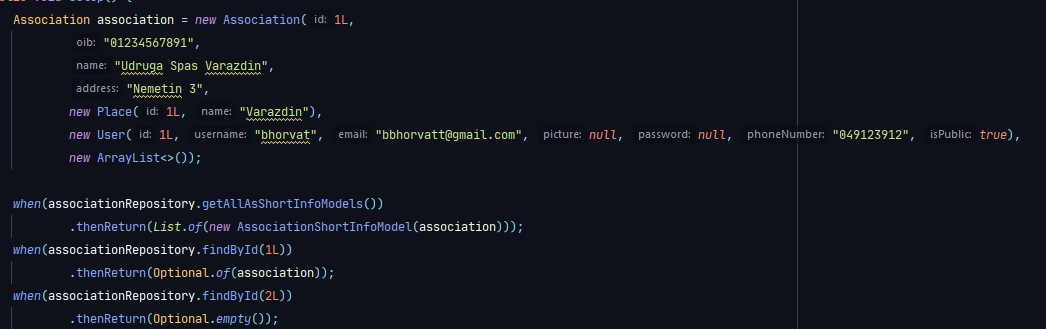
\includegraphics[width=\linewidth]{slike/Testovi-12.png}
		\centering
		\caption{Postavljanje testnih podataka za testiranje AssociationControllera}
		\label{fig:testovi12}
	\end{figure}


	\noindent Na API poziv "/api/association" šaljemo zahtjev za  dohvat svih udruga. Očekivani rezultat je statusni kod 200.

	\begin{figure}[H]
		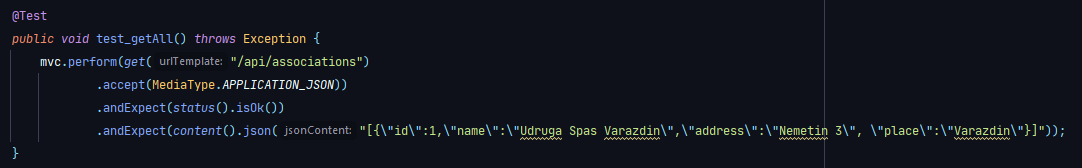
\includegraphics[width=\linewidth]{slike/Testovi-13.png}
		\centering
		\caption{Testiranje dohvata svih udruga}
		\label{fig:testovi13}
	\end{figure}

	\noindent  Na API poziv "/api/association/1" šaljemo zahtjev za dohvat udruge sa šifrom 1. Očekivani rezultat je statusni kod 200.

	\begin{figure}[H]
		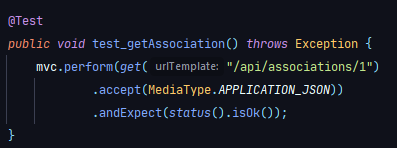
\includegraphics[width=\linewidth]{slike/Testovi-14.png}
		\centering
		\caption{Testiranje dohvata odabrane udruge}
		\label{fig:testovi14}
	\end{figure}

	\noindent Na API poziv "/api/association/2" šaljemo zahtjev za dohvat udruge sa šifrom 2. Očekivani rezultat je statusni kod 400.

	\begin{figure}[H]
		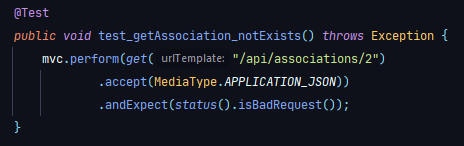
\includegraphics[width=\linewidth]{slike/Testovi-15.png}
		\centering
		\caption{Testiranje dohvata udruge koja ne postoji}
		\label{fig:testovi15}
	\end{figure}

	\eject

	\noindent Slijede rezultati navedenih testova.

	\begin{figure}[H]
		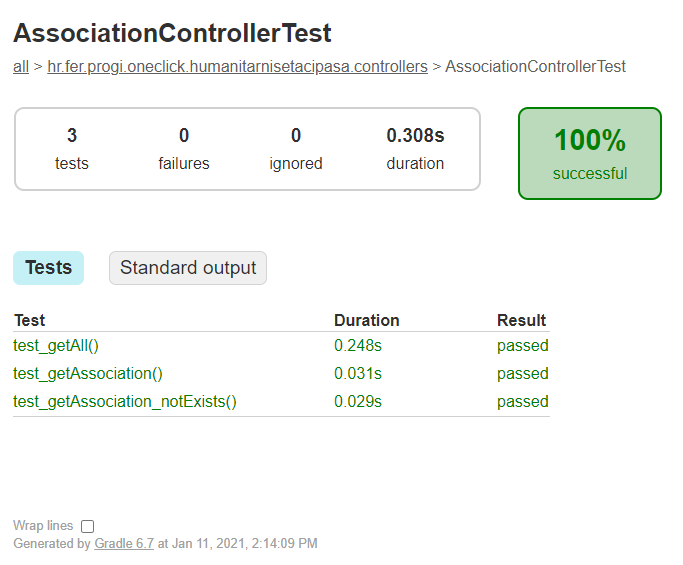
\includegraphics[width=\linewidth]{slike/Testovi-17.png}
		\centering
		\caption{Rezultati testiranja AssociationControllera}
		\label{fig:testovi17}
	\end{figure}
	
	\eject

	\subsection{Ispitivanje sustava}
	
	\noindent Ulaz za prvi test je nevaljano korisničko ime i lozinka. Očekivani rezultat je prikazivanje poruke "Pogrešni podaci za prijavu!".
	
	\begin{figure}[H]
		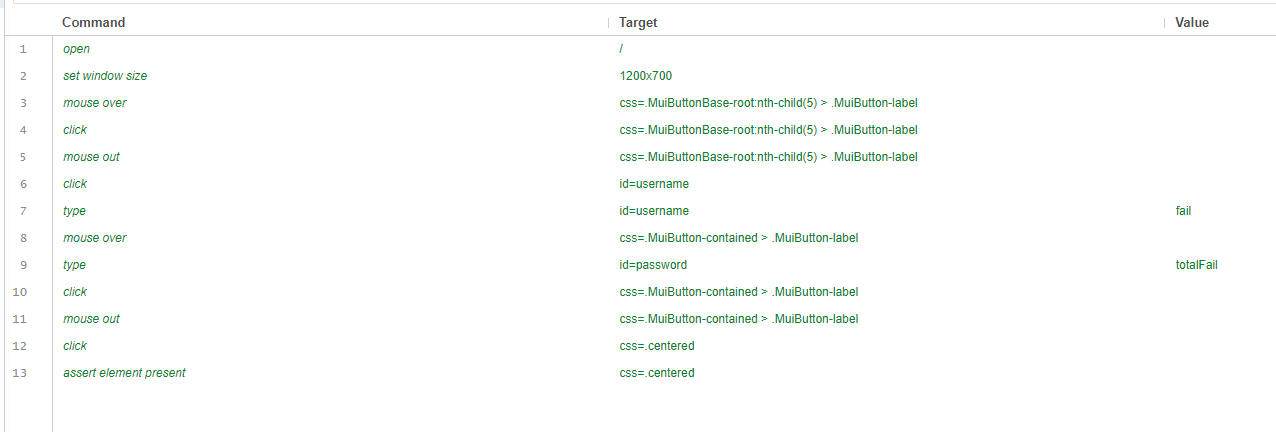
\includegraphics[width=\linewidth]{slike/front-testovi-1.png}
		\centering
		\caption{Koraci prvog testa}
		\label{fig:fronttestovi1}
	\end{figure}
	
	\noindent \newline Rezultat prvog testa je prikaz poruke "Pogrešni podaci za prijavu!".

	\begin{figure}[H]
		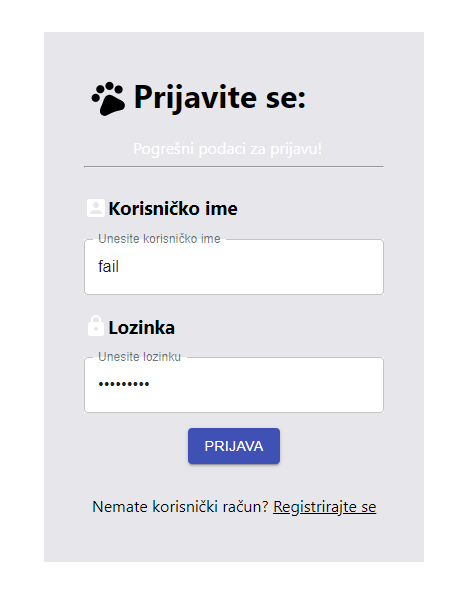
\includegraphics [width=0.50\linewidth]{slike/front-testovi-2.png}
		\centering
		\caption{Rezultat prvog testa}
		\label{fig:fronttestovi2}
	\end{figure}

	\eject

	\noindent Ulaz za drugi test su ispravni podaci. Očekivani rezultat je prijava u sustav.

	\begin{figure}[H]
		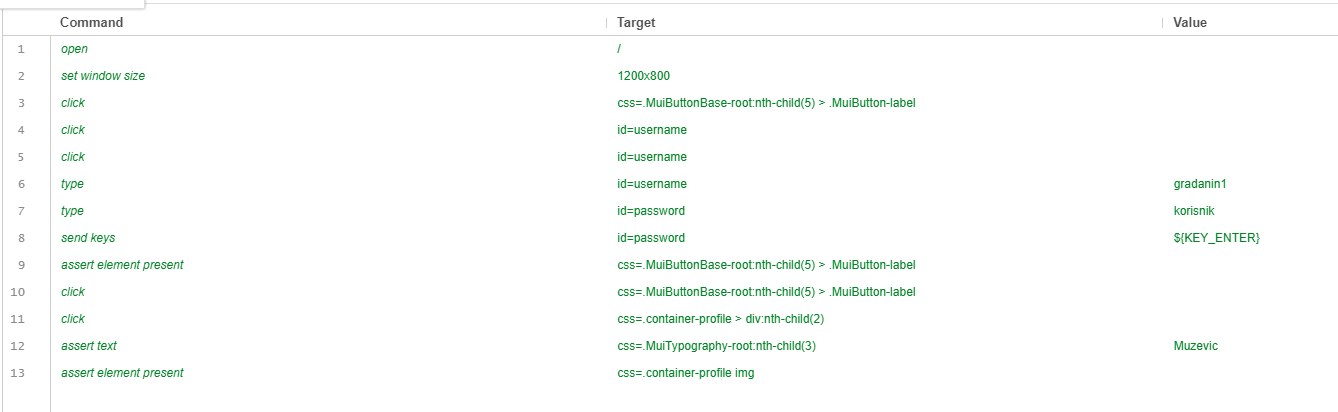
\includegraphics[width=\linewidth]{slike/front-testovi-3.png}
		\centering
		\caption{Koraci drugog testa}
		\label{fig:fronttestovi3}
	\end{figure}

	\noindent \newline Rezultat drugog testa je prijava u sustav s danim korisničkim imenom i lozinkom.

	\begin{figure}[H]
		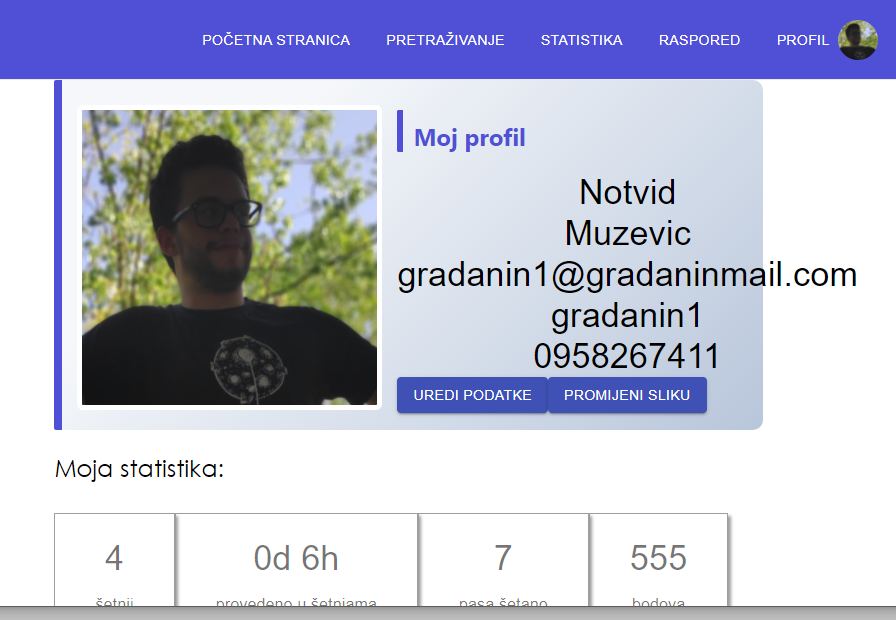
\includegraphics[width=0.8\linewidth]{slike/front-testovi-4.png}
		\centering
		\caption{Rezultat drugog testa}
		\label{fig:fronttestovi4}
	\end{figure}

	\eject

	\noindent Ulaz za treći test su podaci za registraciju. Očekivani rezultat je registracija u sustav.

	\begin{figure}[H]
		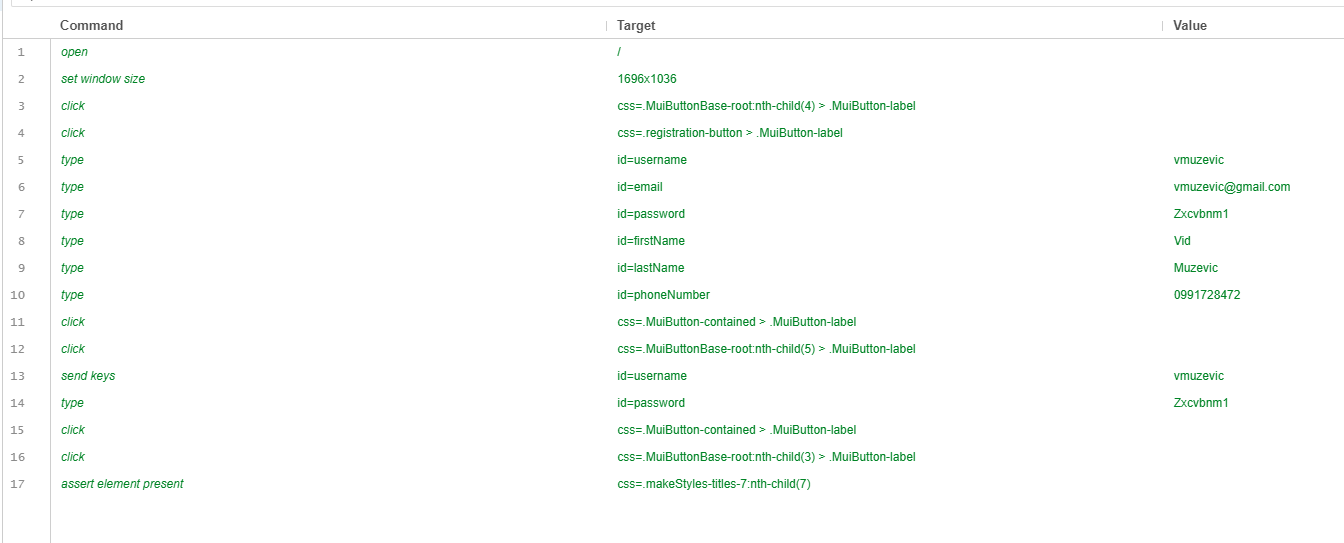
\includegraphics[width=\linewidth]{slike/front-testovi-5.png}
		\centering
		\caption{Koraci trećeg testa}
		\label{fig:fronttestovi5}
	\end{figure}

	\noindent \newline Rezultat trećeg testa je registracija u sustav s danim podacima.

	\begin{figure}[H]
		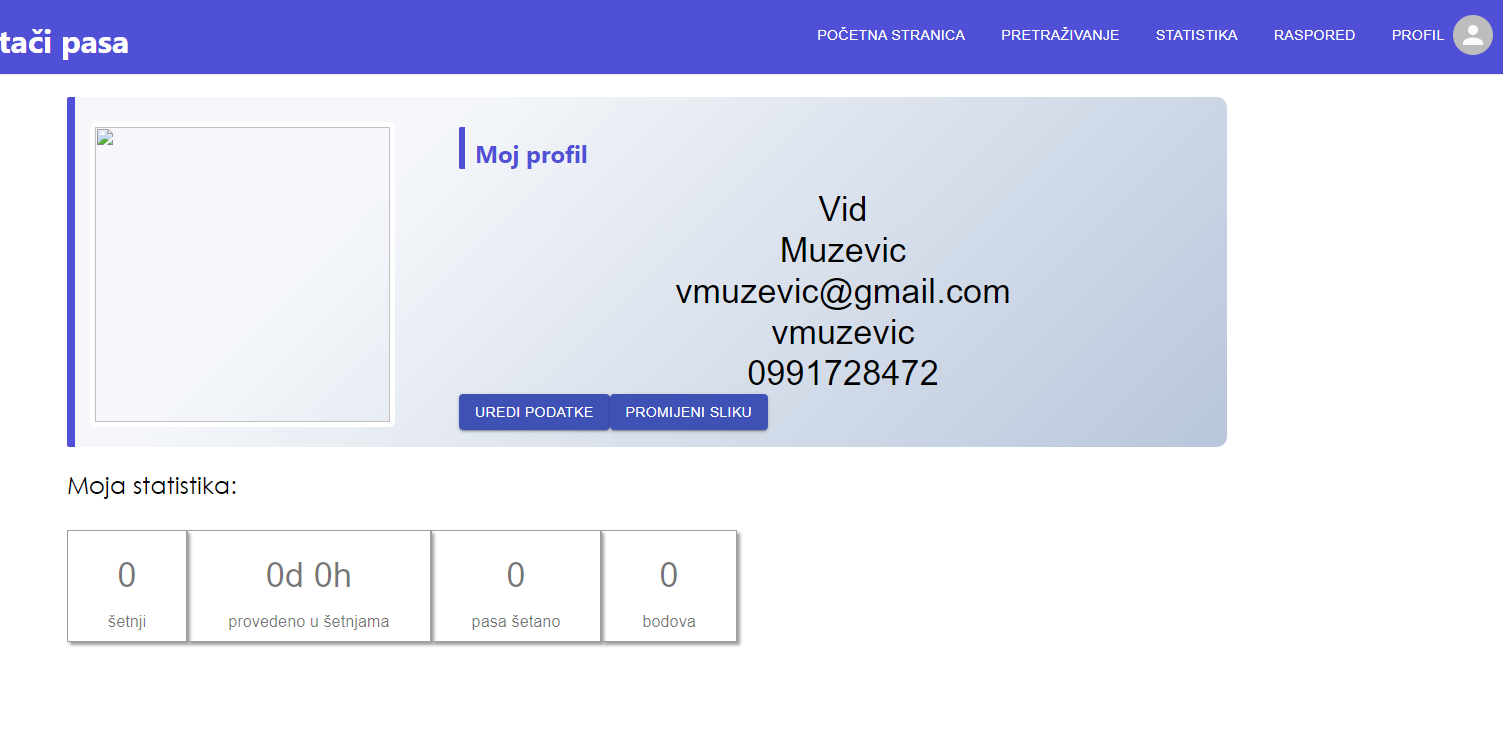
\includegraphics[width=0.9\linewidth]{slike/front-testovi-6.png}
		\centering
		\caption{Rezultat trećeg testa}
		\label{fig:fronttestovi6}
	\end{figure}

	\eject

	\noindent Ulaz za četvrti test su podaci koje želimo urediti, tj. promijeniti njihovu vrijednost. Očekivani rezultat su promijenjeni podaci na stranici profila.

	\begin{figure}[H]
		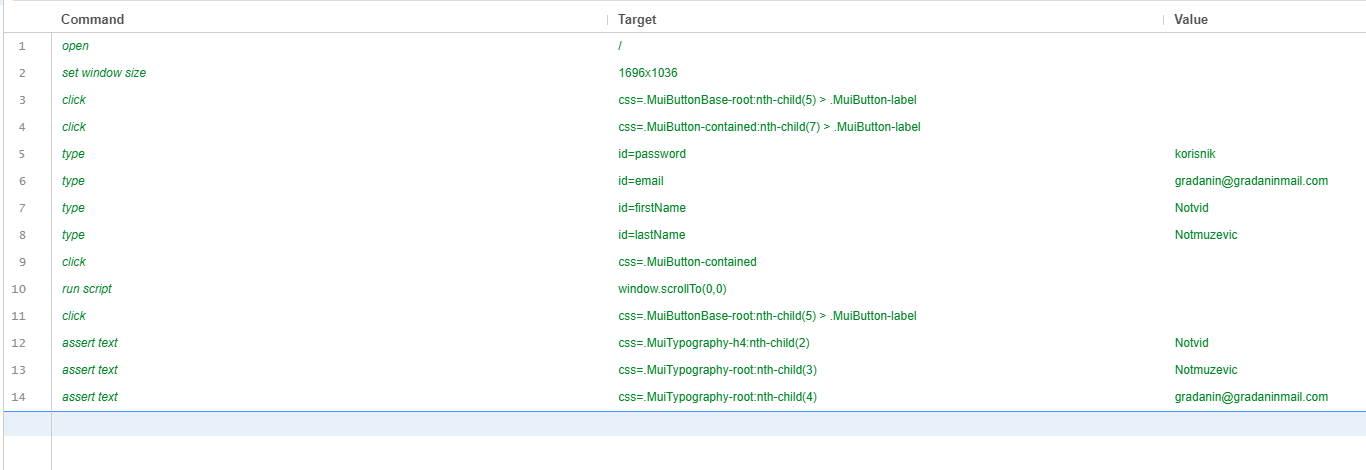
\includegraphics[width=\linewidth]{slike/front-testovi-7.png}
		\centering
		\caption{Koraci četvrtog testa}
		\label{fig:fronttestovi7}
	\end{figure}

	\noindent \newline Rezultat četvrtog testa su promijenjeni podaci na stranici profila.

	\begin{figure}[H]
		
\includegraphics[width=\linewidth]{slike/front-testovi-8.png}
		\centering
		\caption{Rezultat četvrtog testa}
		\label{fig:fronttestovi8}
	\end{figure}

	\eject

	\noindent Ulaz petog testa su podaci za prijavu šetnje, tj. datum, vrijeme početka i trajanje šetnje. U testu se odabir datuma i vremena šetnje provodi klikanjem na elemente za odabir datuma i vremena. Očekivani rezultat je prijava šetnje.

	\begin{figure}[H]
		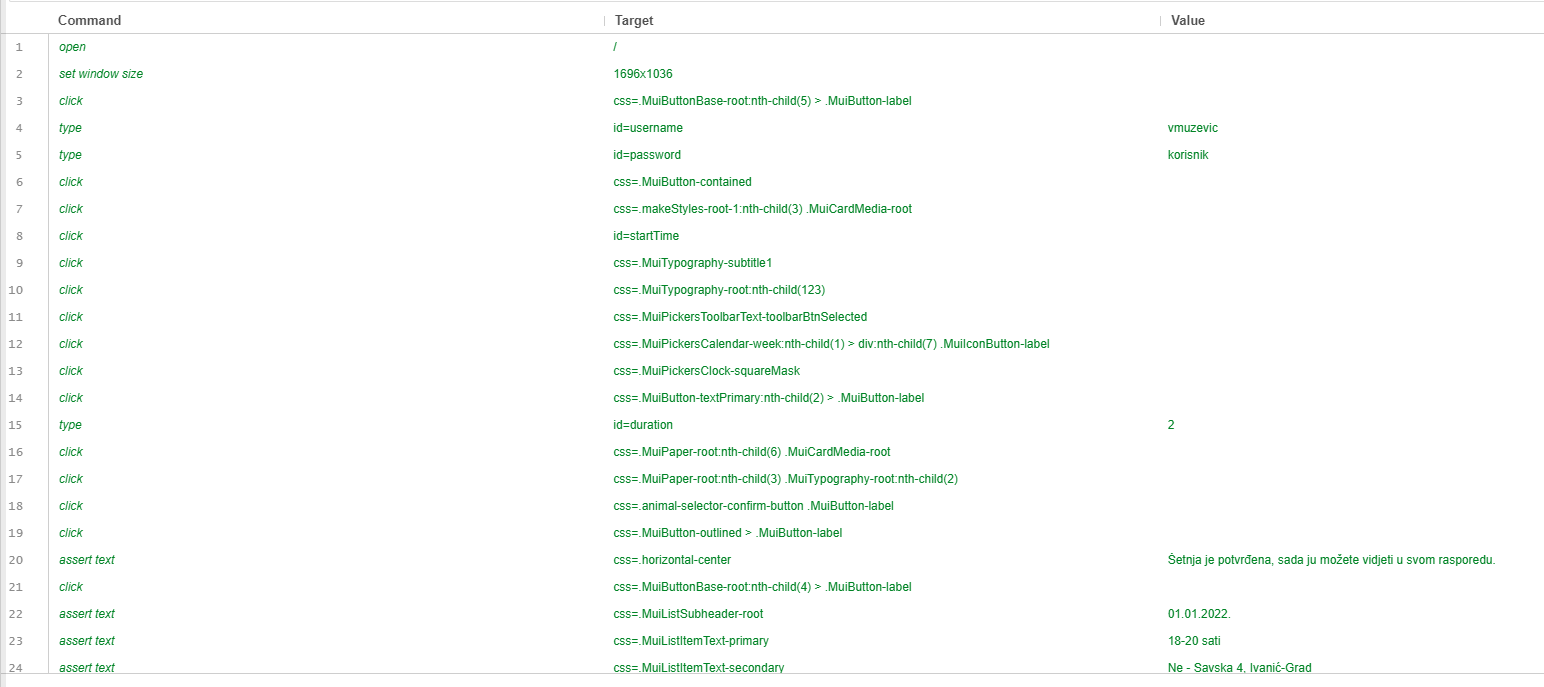
\includegraphics[width=\linewidth]{slike/front-testovi-9.png}
		\centering
		\caption{Koraci petog testa}
		\label{fig:fronttestovi9}
	\end{figure}

	\noindent \newline Rezultat petog testa je prijavljena šetnja koja se može vidjeti u rasporedu.

	\begin{figure}[H]
		
\includegraphics[width=\linewidth]{slike/front-testovi-10.png}
		\centering
		\caption{Rezultat petog testa}
		\label{fig:fronttestovi10}
	\end{figure}

	\eject

	\noindent Ulaz u šesti test su podaci o novoj životinji koju se želi dodati na stranicu udruge. Pretpostavka je da smo prijavljeni u sustav kao udruga. Očekivani rezultat je dodana životinja na stranicu udruge.

	\begin{figure}[H]
		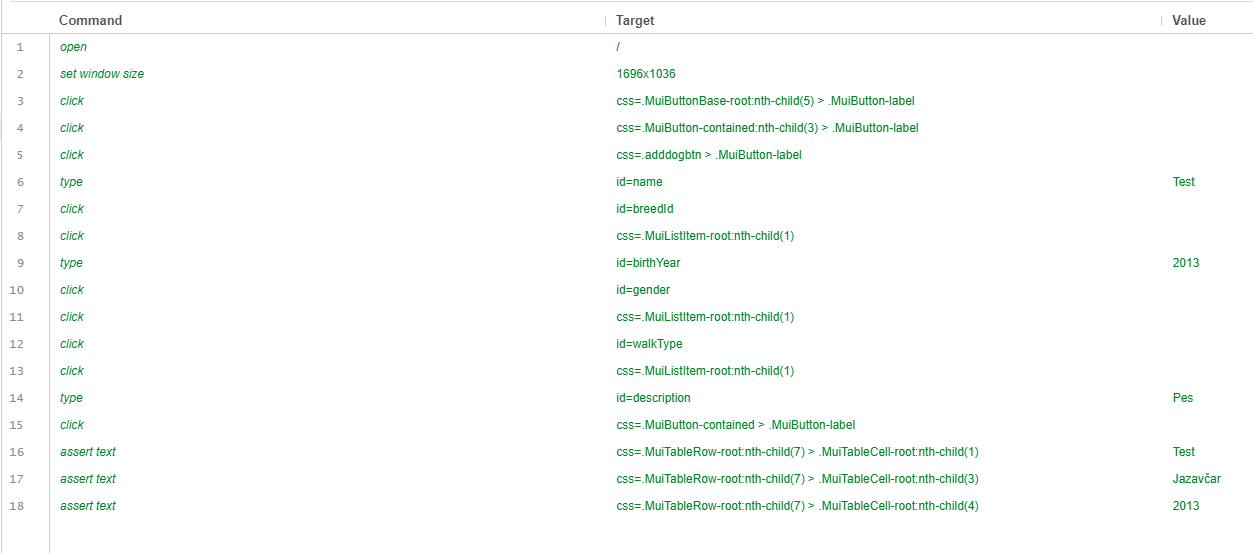
\includegraphics[width=\linewidth]{slike/front-testovi-11.png}
		\centering
		\caption{Koraci šestog testa}
		\label{fig:fronttestovi11}
	\end{figure}

	\noindent \newline Rezultat šestog testa je dodana životinja na stranicu udruge.

	\begin{figure}[H]
		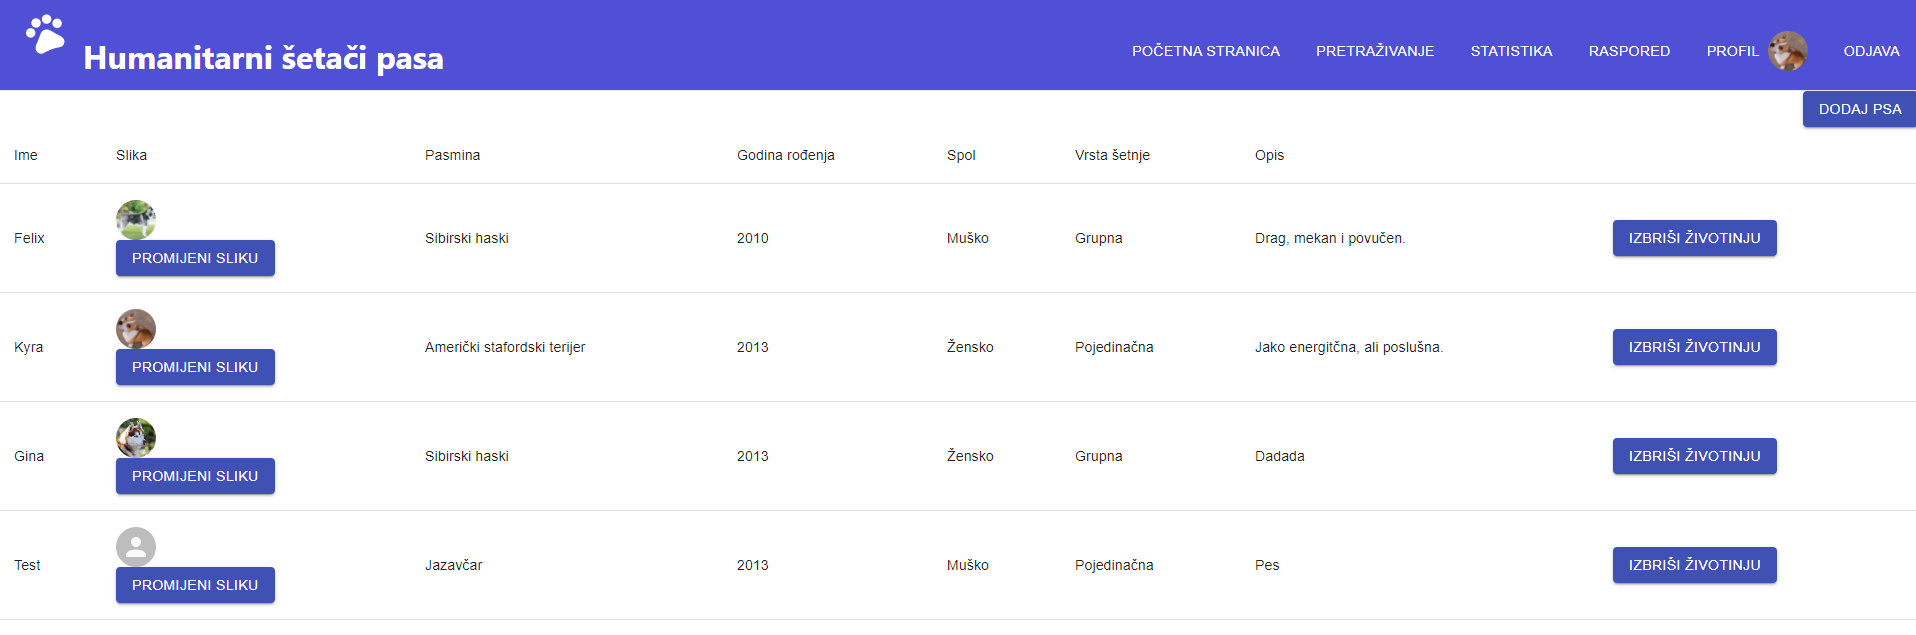
\includegraphics[width=\linewidth]{slike/front-testovi-12.png}
		\centering
		\caption{Rezultat šestog testa}
		\label{fig:fronttestovi12}
	\end{figure}

	\eject

	\noindent Ulaz sedmog testa je klik na gumb "Izbriši životinju". Očekivani rezultat je brisanje životinje dodane u prethodnom testu.

	\begin{figure}[H]
		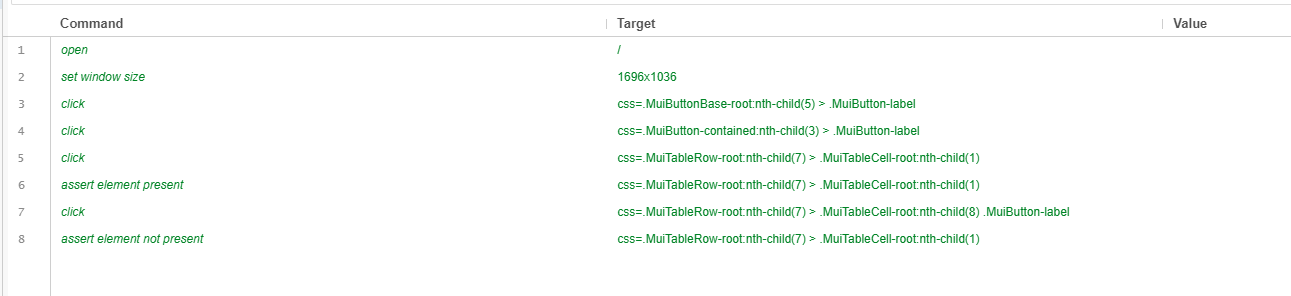
\includegraphics[width=\linewidth]{slike/front-testovi-13.png}
		\centering
		\caption{Koraci sedmog testa}
		\label{fig:fronttestovi13}
	\end{figure}

	\noindent \newline Rezultat sedmog testa je brisanje životinje dodane u prethodnom testu.

	\begin{figure}[H]
		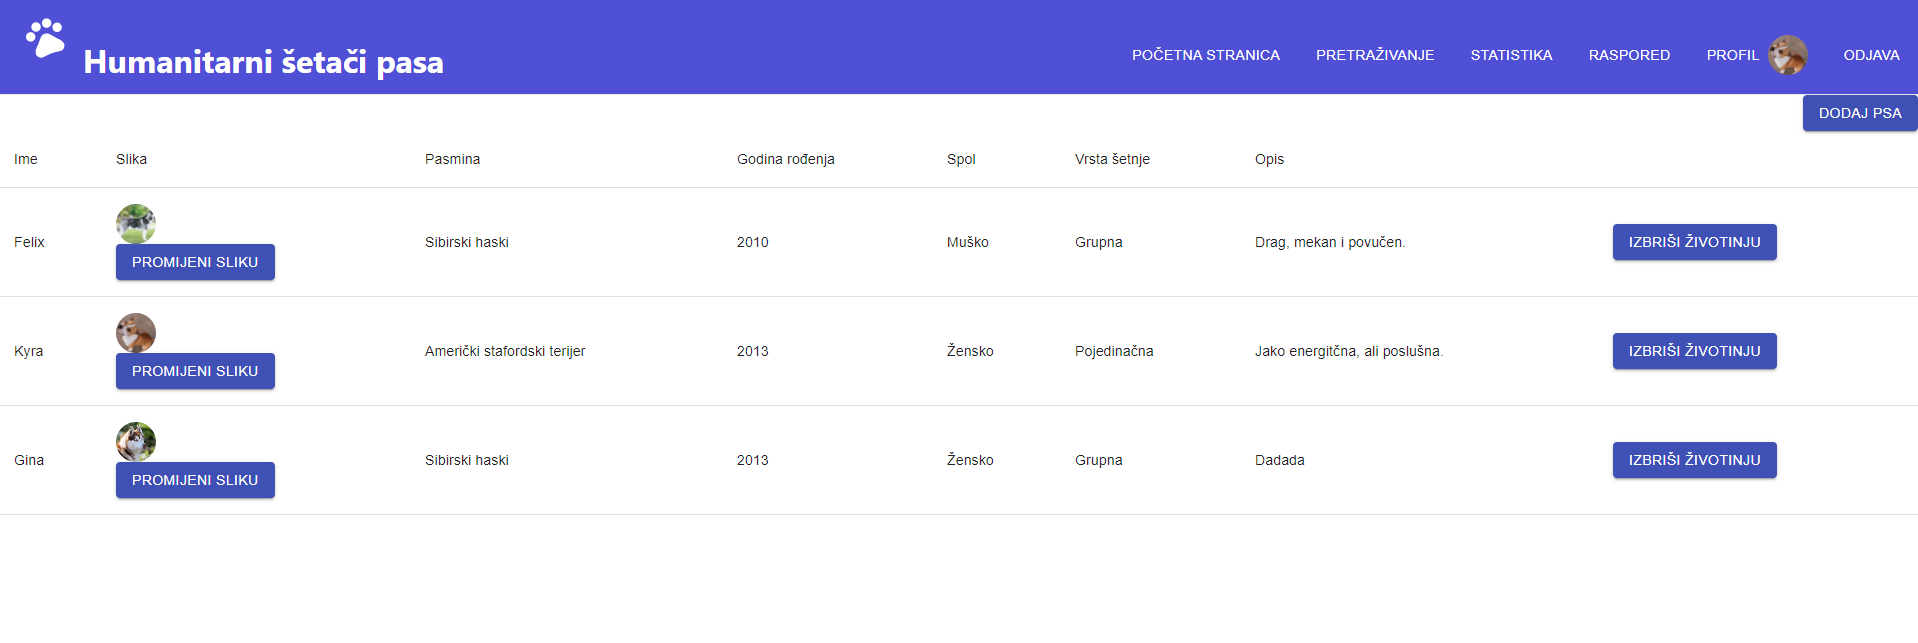
\includegraphics[width=\linewidth]{slike/front-testovi-14.png}
		\centering
		\caption{Rezultat sedmog testa}
		\label{fig:fronttestovi14}
	\end{figure}
	
	\eject
	
	\section{Dijagram razmještaja}
	\begin{figure}[H]
		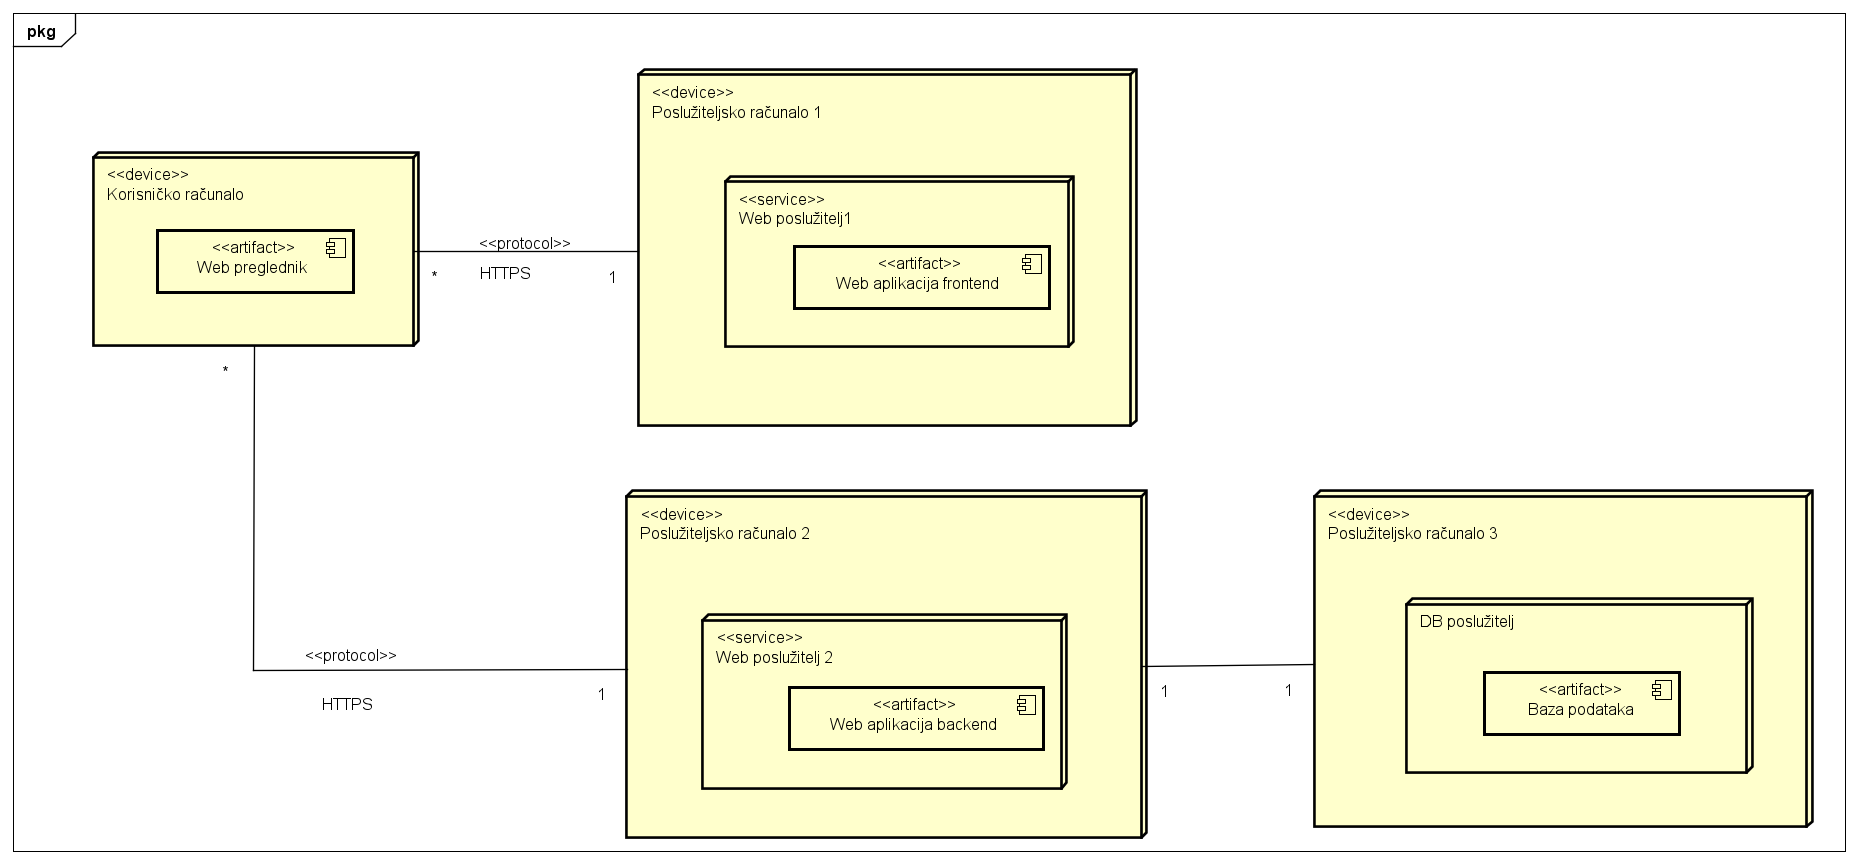
\includegraphics[width=\linewidth]{slike/DeploymentDiagram0.png}
		\centering
		\caption{Dijagram razmještaja}
		\label{fig:dijagramrazmještaja}
	\end{figure}
\eject
\section{Upute za puštanje u pogon}

Za puštanje aplikacije u pogon, ponajprije treba napraviti račun na besplatnoj usluzi za deploy aplikacija - Heroku.
Nakon toga treba napraviti nove projekte i dodati dodatke u same projekte. Odlučili smo se napraviti dva nova projekta, jedan za backend te jedan za frontend.
Kod deploya za backend potrebno je povezati bazu podataka i instalirati ju kao dodatak projektu.
\begin{figure}[H]
	
\includegraphics[width=\linewidth]{slike/heroku-backend.png}
	\centering
	\caption{Povezivanje baze podataka na backend projekt}
	\label{fig:postgresqlbackend}
\end{figure}
Za bazu podataka odlučili smo koristiti PostgreSQL koju je pritom bilo potrebno instalirati na vlastiti operacijski sustav. Nakon dodavanja baze na backend projekt bilo je potrebno tu istu bazu povezati sa našom aplikacijom. Kako bismo to učinili, na vlastitom backend projektu morali smo promijeniti application.properties datoteku. U toj datoteci morali smo promijeniti korisničko ime, lozinku i poveznicu na bazu podataka. Nakon toga baza je bila spremna za punjenje podatcima. Uz to smo dodali i datoteku application-local.properties kako bismo samu aplikaciju mogli pokretati i preko vlastitog localhosta. 
Za izradu frontend dijela projekta koristili smo React, stoga je u sam projekt bilo potrebno dodati buildpack kako bi se instalirale ovisnosti s obzirom na React.
\begin{figure}[H]
	
\includegraphics[width=\linewidth]{slike/heroku-frontend.png}
	\centering
	\caption{Povezivanje Reacta na frontend projekt}
	\label{fig:reactfrontend}
\end{figure}
Nakon dodavanja backenda i frontenda dodali smo još i pipelineove koji su nam olakšavali deployment na Heroku. Pipelineovi su se pokretali izvršavanjem .gitlab-ci.yml datoteke u samom korijenu dokumenta. Za njihovo izvršavanje bilo je potrebno postaviti varijable na gitlabu pomoću kojih smo pristupali backendu i frontendu na Heroku.
\begin{figure}[H]
	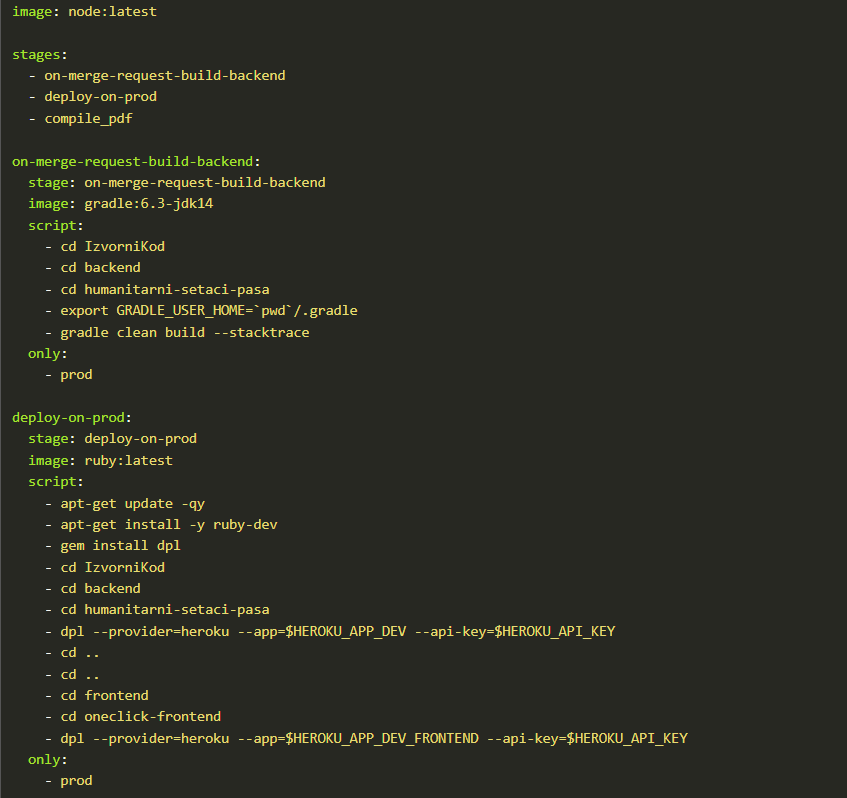
\includegraphics[width=\linewidth]{slike/heroku-cicd.png}
	\centering
	\caption{Datoteka .gitlab-ci.yml korištena kod deploymenta}
	\label{fig:gitlabci}
\end{figure}
Uz pipelineove za deploy dodali smo i jedan za generiranje pdf dokumenta koji je latex dokument pretvorio u pdf koji smo mogli preuzeti. Na taj smo način bili sigurni da se slučajno nije dogodila pogreška prilikom pisanja dokumentacije.
Svi ovi pipelineovi omogućili su nam da prilikom mergea na granu koju smo zadali provjerimo je li došlo do pogreške te zatim aplikaciju uspješno deployamo na Heroku.
\begin{figure}[H]
	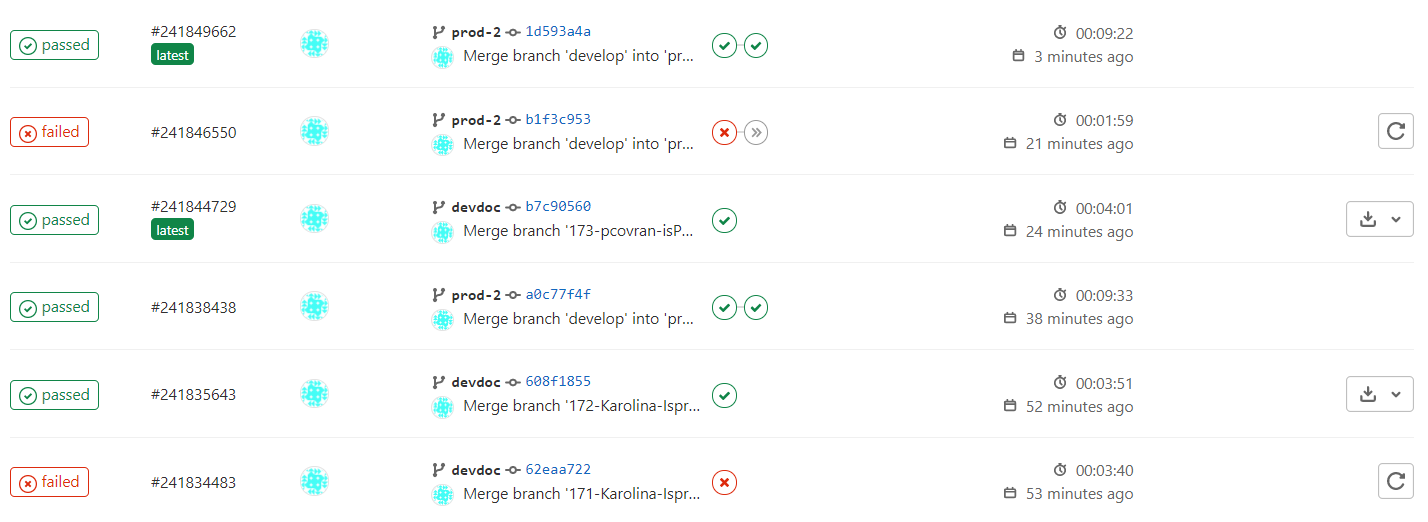
\includegraphics[width=\linewidth]{slike/heroku-pipelines.png}
	\centering
	\caption{Primjer pipelineova}
	\label{fig:pipelines}
\end{figure}